\section{Stability analysis}

\subsection{Stabilite d'un etat d'equilibre}
\com{Plan : Obtention du critere sL permettant de savoir si un etat d'equilibre donne est stable ou non}

The macroscopic model consists in an aggregation-diffusion equation with nonlocal terms which are related to interaction between neighbors \notok{of the same family and ones of the other family}.
In this section we perform a linear stability analysis of macroscopic model with logistic term in order to explore the formation of aggregations. In the following, appearance of clusters in the model will be characterized by the stability of the homogeneous states. \\
%in order to identify also phase transitions of the homogeneous steady-state. \\
We linearize around the homogeneous states, i.e. we consider the constant steady states $\bfA$ and $\bfB$ which satisfy \eqref{MacroModel}. 
%(forgetting the bars):
% 	\begin{equation}
% \begin{cases}
% \p_t f^{A}-  \nabla \cdot (f^A\nabla_x(\Phi^{AA}* f^A)) - \nabla \cdot (f^A \nabla_x \Phi^{AB}*f^B) - D_A \Delta_x f^A - \nu^{A}f^A\left( 1-\frac{f^A+f^B}{f^{*}} \right)=0 \\
% 
% \p_t f^{B}-  \nabla \cdot (f^B\nabla_x(\Phi^{BB}* f^B)) - \nabla \cdot (f^B \nabla_x \Phi^{BA}*f^A) - D_A \Delta_x f^A - \nu^{B}f^B\left( 1-\frac{f^A+f^B}{f^{*}} \right)=0
% \end{cases}
% \end{equation}
Since $\bfA,\bfB$ do not depend on time and space, we can reduce the system to:%since we know that 
%$\nabla \cdot (\bfA \nabla (\Phi^{AA} * \bfA)) =0 $, all derivative terms are zero.
% It leads us to following equations:
\begin{equation}
\begin{cases}
	\nu^{A}\bfA\left( 1-\frac{\bfA+\bfB}{f^{*}} \right)=0 \\
	\nu^{B}\bfB\left( 1-\frac{\bfA+\bfB}{f^{*}} \right)=0
\end{cases}
\end{equation}
% The first equation is satisfied either when $\bfA=0$ or $f^A\left( 1-\frac{f^A+f^B}{f^{*}} \right)=0$ and the second one is satisfied by $\bfB=0$ or $f^B\left( 1-\frac{f^A+f^B}{f^{*}} \right)=0$. In this case we obtain the following relation:
We deduce that the non-trivial constant steady states are defined through the relation:
\begin{equation}
 \bfA+\bfB=f^*,
\end{equation}
which means that, at the homogeneous states, we have reached the maximum carrying capacity. \com{Mentionner difference avec le modele sans logistique : infinite de solutions; $f^A,f^B$ ne sont plus des densites de probas?}

We perform a stability analysis, using perturbation terms and Fourier transform as in \cite{twoparticule}, in order to understand if a possible perturbation can have effects on our model and it corresponds to the appearance of some clusters. \\
After computation, we obtain the following system:
\begin{align}
\p_t \begin{pmatrix} \hat{f}^A \\ \hat{f}^B
\end{pmatrix}(y,t)=M(y)\begin{pmatrix} \hat{f}^A \\ \hat{f}^B
\end{pmatrix}(y,t)
\end{align}
with matrix $M$ defined as:

\begin{align}
M(y)=
 \begin{pmatrix} -|y|^2(2\pi\bfA\hPAA(y)+D_A)-\nu_{b}^A\frac{\bfA}{f^*} & -|y|^22\pi\bfA\hPAB(y)-\nu_{b}^A\frac{\bfA}{f^*} \\ 
-|y|^2\bfB\hPBA(y)-\nu_{b}^B\frac{\bfB}{f^*} & -|y|^2(2\pi\bfB\hPBB(y)+D_B)-\nu_{b}^B\frac{\bfB}{f^*} 
\end{pmatrix}.
\end{align}

%This is a linear ODE system, hence its solution is:
%$$
%\begin{pmatrix} \hat{f}^A \\ \hat{f}^B
%\end{pmatrix}(y,t)=c_1(y)exp^{\la_1(y)t}u_1(y)+c_2(y)exp^{\la_2(y)t}u_2(y).
%$$
%where $\la_1(y), \la_2(y)$ are the eigenvalues of the matrix and $u_1(y),u_2(y)$ the corrisponding eigenvectors. 


In general case, the constant steady state will be stable only if the eigenvalues of the matrix $M(y)$ are both negative, otherwise it will be unstable \com{ce n'est pas plutot la partie reelle des vp?}. Since we know that $det(M(y))=\la_1 \cdot \la_2$ and $tr(M(y))=\la_1+\la_2$, with $\la_1(y), \la_2(y)$ eigenvalues, the stability occurs only if:
\[det(M(y))>0\quad \text{and} \quad tr(M(y))<0\]
At first we compute the trace of matrix $M(y)$:
\begin{equation}
 tr(M(y))=-|y|^2(2\pi\bfA\hPAA(y)+D_A)-\nu_{b}^A\frac{\bfA}{f^*}-|y|^2(2\pi\bfB\hPBB(y)+D_B)-\nu_{b}^B\frac{\bfB}{f^*}
\end{equation}
As in \cite{twoparticule}, we consider the following assumption:
\begin{hypo}\label{hypo_rep}
 The intraspecies links generate repulsive interactions, i.e $\KAA>0$ and $\KBB>0$.
\end{hypo}
We can easily note that under Hypothesis \ref{hypo_rep}, the trace is always negative.
Then we compute the determinant of matrix $M(y)$:
%\begin{align}
%det(M(y))=|y|^4 \left[ (\bfA 2\pi \hPAA +D_A)(\bfB 2\pi \hPBB +D_B) - \bfA \bfB 4 \pi^2 \hPAB \hPBA \right] + \\
%+|y|^2 \left[ \nu_b^B \frac{\bfB}{f^{*}}(\bfA 2\pi \hPAA + D_A -\bfA 2\pi \hPAB) - \nu_b^A \frac{\bfA}{f^{*}}(\bfB 2\pi \hPBB + D_B -\bfB 2\pi \hPBA)   \right].
%\end{align}
\begin{equation}
\begin{split}
det(M(y))&= |y|^4 \left[ (\bfA 2\pi \hPAA +D_A)(\bfB 2\pi \hPBB +D_B) - \bfA \bfB 4 \pi^2 \hPAB \hPBA \right] + \\
&+|y|^2 \left[ \nu_b^B \frac{\bfB}{f^{*}}(\bfA 2\pi \hPAA + D_A -\bfA 2\pi \hPAB) - \nu_b^A \frac{\bfA}{f^{*}}(\bfB 2\pi \hPBB + D_B -\bfB 2\pi \hPBA)   \right].
\end{split}
\end{equation}
The first part with term in $|y|^4$ is exactly the determinant computed in \cite{twoparticule} without logistic term. The second one is due to the introduction of logistic growth. \\
 We introduce a parameter $s \in \mathbb{R}$ and we scale the interspecies (heterotypic) link potential intensities such that $\kappa^{ST}=s \widetilde{\kappa}^{ST} $. \com{Detailler plus le s. Ecrire det(M) avec s?}
\begin{hypo}\label{hypo_rep2}
 The interspecies links interactions are both repulsive or both attractive, i.e $\KAB\KBA>0$. \com{A verifier}
\end{hypo}
Following the same workflow  and approach of \cite{twoparticule}, we find the critical value $\sL$, such that if $s> \sL$ and under Hypothesis \ref{hypo_rep2} we should observe the formation of clusters. In the case of model with logistic term we have:
% \begin{equation}
% \sL=\frac{(24 D_A+c'^{AA})\nu_{b}^{B}\bar{f}^{B}+(24 D_B+c'^{BB})\nu_{b}^{A}\bar{f}^A}{\nu_{b}^{B}\bar{f}^B\tilde{c}'^{AB}+\nu_{b}^{A}\bar{f}^A\tilde{c}'^{BA}},
% \end{equation}
\begin{equation}
\sL=\frac{(24 D_A+c'^{AA}\bfA)\nu_{b}^{B}\bar{f}^{B}+(24 D_B+c'^{BB}\bfB)\nu_{b}^{A}\bar{f}^A}{\nu_{b}^{B}\bar{f}^B\tilde{c}'^{AB}\bfA+\nu_{b}^{A}\bar{f}^A\tilde{c}'^{BA}\bfB},
\end{equation}
with $c'^{ST}=\frac{2\pi k^{ST} \nu_c^{ST} R^{4}}{\nu_d^{ST}}$, $S,T \in \{ A,B \}$.
%$c'^{ST}=\frac{2\pi k^{ST} \bfS \nu_c^{ST} R^{4}}{\nu_d^{ST}}$, $S,T \in \{ A,B \}$
%As did in [cit], we introduce a parameter $s\in \mathbb{R}$ to scale the interspecies potential intensities such that $\ka^{ST}=s\tilde{\ka}^{ST} $.

\com{Remarque sur les cas d'extinction de pop? Analyse de stab tjs valide? On obtient au moins une vp nulle dans la matice donc instabilité?}

\subsection{Aggregation ou non}
\com{Plan : Comportement globale de sL en fonction de fA : on a toujours des etats stables. Graphe de sL avec des valeurs raisonnables : on peut assurer que la plupart des etats stationnaires sont instables et donc aggregation si une population ne domine pas l'autre au temps initial.}

The critical value $\sL$ define the stability of a given steady state. Because there is an infinity of steady states, in order to ensure the apparition of clusters, we have to ensure that all steady states are unstable.

%We set $c'^{AA}=k_1 \bfA, \ c'^{BB}=k_2\bfB, \ c'^{AB}=k_3\bfA, \ c'^{BA}=k_4\bfB$.
By $\bar{f}^B=f^*-\bar{f}^A$ we rewrite the following $s^*_{L}$:

% \begin{equation}
% \sL=\frac{(24 D_A+k_1\bfA)\nu_{b}^{B}(f^*-\bfA)+(24 D_B+k_2(f^*-\bfA))\nu_{b}^{A}\bar{f}^A}{\nu_{b}^{B}(f^*-\bfA)k_3\bfA+\nu_{b}^{A}\bar{f}^Ak_4(f^*-\bfA)}.
% \end{equation}

\begin{equation}
\sL=\frac{(\nu_{b}^{B}c'^{AA}+\nu_{b}^{A}c'^{BB})\bfA(f^*-\bfA)+(24 D_B\nu_{b}^{A}-24 D_A\nu_{b}^{B})\bfA+24 D_A\nu_{b}^{B}f^*}{\bfA(f^*-\bfA)(\nu_{b}^{B}\tilde{c}'^{AB}+\nu_{b}^{A}\tilde{c}'^{BA})},
\end{equation}

% To simplify notation, we take into account the following function depending on $\bfA$ and its derivative :
% $$F(\bfA)=\frac{\a \bfA + \b (\bfA)^2 + \g}{\d \bfA + \eps(\bfA)^2}, \quad\quad 
% \frac{\p F(\bfA)}{\p \bfA}=\frac{(\bfA)^2(\b \d-\a \eps)-2\eps \g \bfA - \g\d}{(\d \bfA+\eps (\bfA)^2)^2},$$ 
% with parameters 
% \begin{equation}
% \begin{split}
% \a=& 24D_B \nu_b^A -24 D_A \nu_b^B +k_1 \nu_b^B f^* + k_2 \nu_b^A f^*, \quad
% \b=-k_1 \nu_b^B -k_2 \nu_b^A, \\
% \g=& 24 D_A \nu_b^B f^*, \quad 
% \d= k_3\nu_b^B f^*+k_4 \nu_b^A f^*, \quad
% \eps= -\nu_b^B k_3-	\nu_b^A k_4.
% \end{split}
% \end{equation}
% \begin{remark}
% 	The condition $\d \bfA + \eps (\bfA)^2 \ne 0 $ in $F(\bfA)$ ensures the existence of function, in other words we get  $\bfA \ne 0 $ or $\bfA \ne -\frac{\d}{\eps}=f^*$. 
% \end{remark}

To study the stability of all steady states we study the variation of $\sL$ as a function of $\bfA\in[0,f^*]$.

\com{Limite en 0 et $f^*$, sous H1 et H2, sL>0}

We are looking for the minimum of function $\sL$, i.e the zero points of $\frac{\p \sL(\bfA)}{\p \bfA}$. After computation we can conclude: \com{Expression de la dérivée? Distinguer le cas $D_A \nu_b^B -\nu_b^A D_B=0$}
\begin{equation}
\bfA_{min}=\frac{f^*(D_A \nu_b^B \pm \sqrt{D_A D_B \nu_b^B \nu_b^A})}{D_A \nu_b^B -\nu_b^A D_B}.
\end{equation}

\com{Graphe de $\sL$. Conclusion : certains etats d'equilibre sont toujours stables mais avec des parametres raisonnables on un plateau et donc on peut trouver un s si une population ne domine pas l'autre.}

%If we look at those two values, we can find that:
%
%\begin{equation}
% 0<\frac{f^*(D_A \nu_b^B - \sqrt{D_A D_B \nu_b^B \nu_b^A})}{D_A \nu_b^B -\nu_b^A D_B}<f^*.
%\end{equation}
%and
%\begin{equation}
% \left|\frac{f^*(D_A \nu_b^B + \sqrt{D_A D_B \nu_b^B \nu_b^A})}{D_A \nu_b^B -\nu_b^A D_B}\right|>f^*.
%\end{equation}

\subsection{Comparaison deux modeles}
\com{Plan : Pas de comparaison simple : exemples}

\com{Expliquer pourquoi la comparaison est difficile. Un etat stat contre une infinite. Impossibilite de prevoir la masse totale de A et B a l'equilibre. On fait une comparaison simple a etat fixe.}
With regard to model without logistic term, we report the following critical value as in \textbf{citation}, in order to do a comparison between the two values: \com{Reecrire sC avec fA et fB.}
$$ s^{*}_{C}= \left[\frac{576}{\tilde{c}'^{AB} \tilde{c}'^{BA}} \left( D_A+\frac{c'^{AA}}{24} \right) \left(D_B+\frac{c'^{BB}}{24} \right) \right]^{\frac{1}{2}}. $$

% We simplify notation as already done, taking in this case:
% \begin{equation}\label{notation}
% \a=24D_Bk_3-24D_Ak_4+k_3k_4f^{*}, \quad \b=k_3k_4, \quad \g=576D_AD_B+24D_Ak_4f^{*}, 
% \d=k_1k_2f^{*}, \quad \eps=k_1k_2.
% \end{equation}
%              
% Then, we can rewrite the value $s^{*}_{C}$ and its derivative with respect to $\bfA$ as: 
% $$ s^{*}_C=F(\bfA)=\left[\frac{\g +\a \bfA - \b (\bfA)^2}{\d \bfA-\eps(\bfA)^2} \right]^{\frac{1}{2}},  \quad \frac{\p F(\bfA)}{\p \bfA}=\frac{1}{2} \frac{(\bfA)^{2}(\eps \a-\d\b)+2\eps\g\bfA-\d\g}{(\g+\a \bfA-\b(\bfA)^2)^{1/2} (\d\bfA-\eps(\bfA)^2)^{3/2} }.  $$
% 
% %We want to find the point that minimizes this function, i.e $\frac{\p F(\bfA)}{\p \bfA}=0$. 
% \begin{remark}
% 	In this case we also consider that $\bar{f}^B=f^*-\bar{f}^A$ and the following relation: $\frac{\d}{\eps}= f^{*}$.
% \end{remark}
We are looking for critical points and we get:
$\bfA= \frac{-2\eps \g \pm \sqrt{\Delta}}{2(\eps \a-\d\b)}=\frac{-2\eps \g \pm \sqrt{\Delta}}{2\eps (\a-f^{*}\b)}.$

 Using \eqref{notation} and simplifying, we arrive at: \com{Expression avec les c au lieu des k. Expression de la derivee. Distinguer cas $D_Bk_3-D_Ak_4=0$}
\begin{equation}
\bfA=\frac{-(24 D_AD_B+D_Ak_4f^{*}) \pm \sqrt{\widetilde{\Delta}}}{D_Bk_3-D_Ak_4}, 
\end{equation}

with $\widetilde{\Delta}=(24D_AD_B+D_Ak_4f^{*})^2+24D_AD_B^{2}k_3f^{*}-24D_A^2D_Bk_4f^{*}+D_A D_B k_3 k_4(f^{*})^{2}-D_A^{2} k_4^2 (f^{*})^2.  $

\noindent Both critical values $s^{*}_C, s^{*}_L$ are markers of instability and we will discuss some simulations to compare them. As remarked in \textbf{citation}, the diffusion and intraspecie repulsion tend to homogeneize the system, then the interspecies forces must be large enough to compensate this aspect. Thanks to stability analysis, we can observe that logistic growth can either support or repress aggregation, depending also on the parameters choice.
We want to explore and discuss some different cases:
(?should we insert table with different cases explored in simulations?)
\begin{figure}
	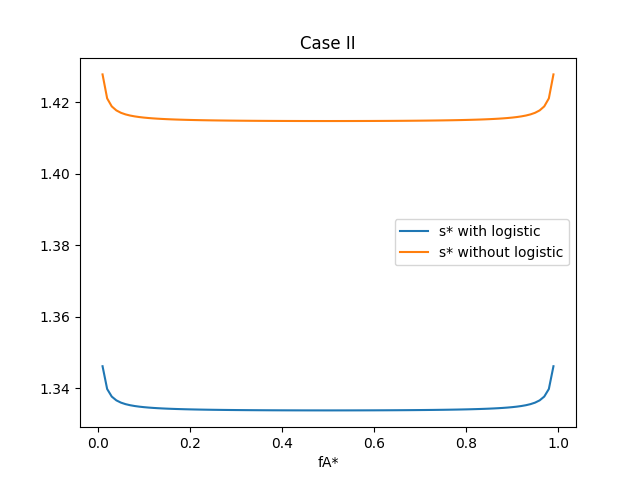
\includegraphics[width=4.5cm]{sstar_caseII}
	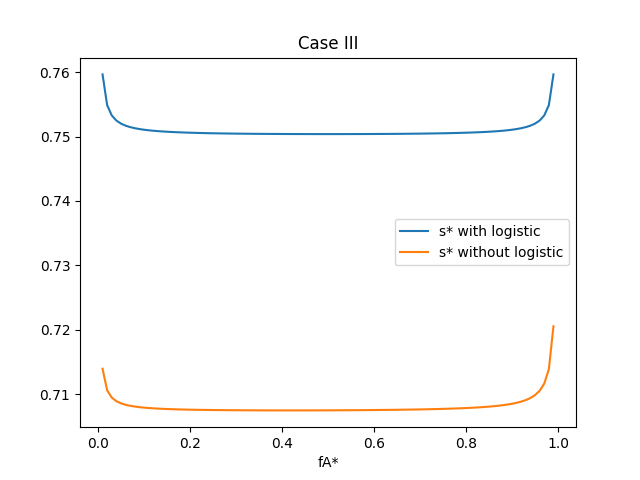
\includegraphics[width=4.5cm]{sstar_caseIII}
	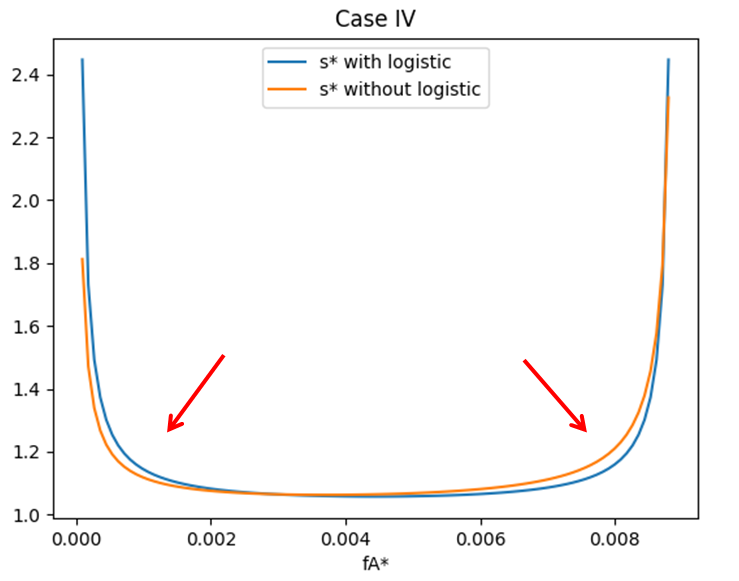
\includegraphics[width=4cm]{caseIVmodi}
	\caption{Placeholder critical values}
\end{figure}


\begin{itemize}
	\item case $s^{*}_{C}<s^*_{L}$. If $s< s^{*}_{c}$ we should observe stability for both model, if $s \in (s^{*}_C, s^{*}_L)$ we should observe instability for model and no aggregates for with logistic one. In the case of $s>s^{*}_{L}$ we expect instability and cell aggregates for both models. 
	\item case $s^{*}_{C}>s^*_{L}$. We should observe the opposite behavior compared to the previous one and instability for logistic model and no aggregates for the other one when  $s \in (s^{*}_L, s^{*}_C)$.
\end{itemize}


In the next section we will discuss some numerical simulations on the individual agent-based model to confirm the results provided by stability analysis.




%%---simulation values---
%	\begin{center}
%	\begin{tabular}{ l |c|c|c| r }
%	\hline
%		Test & $\nu_b^{A}$ & $\nu_b^{B}$ & $s^{*}_{L}$ & s \\ 
%		\hline
%		I &  $10^{-5}$ & $10^{-4} $ & 1.9 & $1.7$ \\ 
%		% II & $5 \cdot 10^{-5}$  & $10^{-4}$ & $1.56$ & $1.51$   \\
%		IIIa & $10^{-4}$  & $10^{-4}$ & $1.39$ & $1.43$ \\
%		IIIb & $10^{-4}$  & $10^{-4}$ & $1.39$ & $1$ \\
%		IIIc & $10^{-4}$  & $10^{-4}$ & $1.39$ & $2$ \\
%		% IV  & $10^{-4}$ & $5\cdot 10^{-5}$ & $1.25$ & $1.35$ \\
%		V & $10^{-4}$ & $10^{-5}$ & $1.09$ & $1.3$ \\
%		
%	\hline
%	\end{tabular}
%	\end{center}







